\documentclass{article}[12 pt]
\usepackage{amssymb}
\usepackage{amsthm}
\usepackage{amsmath}
\usepackage{appendix}
\usepackage{array}
\usepackage{geometry}
\usepackage{enumitem}
\usepackage{graphicx}
\usepackage{subfig}
\usepackage{caption}
\usepackage{url}
\usepackage{float}
\usepackage{pdfpages}
\usepackage{shortvrb}
\usepackage{mathtools}
\usepackage{multirow}
\usepackage{hyperref}
\usepackage{algorithm}
\usepackage[noend]{algpseudocode}

\def\BibTeX{{\rm B\kern-.05em{\sc i\kern-.025em b}\kern-.08em
		T\kern-.1667em\lower.7ex\hbox{E}\kern-.125emX}}

\graphicspath{{"//ece-azare-nas1.ad.ufl.edu/ece-azare-nas/Profile/cmccurley/Desktop/ImageProcessing/HW02/Report/Images/"}}
\geometry{margin=1 in}

\newcommand{\smallvskip}{\vspace{5 pt}}
\newcommand{\medvskip}{\vspace{30 pt}}
\newcommand{\bigvskip}{\vspace{100 pt}}
\newcommand{\tR}{\mathtt{R}}

%===================================================================================================================
\begin{document}
	
\begin{center}
	\textbf{\Large Connor McCurley} \\
	EEE 6512 \qquad \textbf{\large Homework 1 Due September 15, 2018} \qquad Fall 2018 
\end{center}

%===================================================================================================================
\section*{Part I Textbook Questions}

\subsection*{2.5}

Since $\lambda = \frac{c}{\nu}$ , then  $\lambda = \frac{c}{60Hz}$ = $\frac{2.998 \cdot 10^8 m/s}{60Hz}$ = $4.997 \cdot 10^8m$ Therefore, \[ \boxed{\lambda = 4.997 \cdot 10^5 km} \]

\subsection*{2.10}
I can imaging solving the problem presented in 1 of 2 ways (although I'm sure there are many more):
\begin{enumerate}
\item You could take an RGB image of the car over a spot with pure color (i.e. just the color of the car), set a threshold of intensity (close to 255 for an 8-bit image), and check each of the three channels for just the center pixel.  If all three channel's pixels are above the threshold, the car's color is white, otherwise, the color should be the only channel that has an intensity value above the chosen threshold.

\item Additionally, you could just shine a light on the car and measure the wavelength of the reflected beams (since each color in the spectrum has a different wavelength).

\end{enumerate}


\subsection*{2.16}

The two subsets are adjacent with:
\begin{enumerate}
\item 4-adjacency: No 
\item 8-adjacency: Yes
\item m-adjacency: Yes
\end{enumerate}

\subsection*{2.23}

I interpreted "one-dimensional" as meaning the images were stored in vectors.  For the element-wise multiplication to make sense, both vectors must be either row vectors or column vectors with their starting an ending pixels in the same position.  Alternatively, if "one-dimensional" referred to the number of channels, then orientation of the images does not matter as long as the each image's corner pixels are in corresponding locations.

\subsection*{2.39(b)}

Given that the translation matrix is formed by $\begin{bmatrix} 1 & 0 & t_x \\ 0 & 1 & t_y \\ 0 & 0 & 1 \end{bmatrix}$
then, the inverse translation can be performed as 
$\left[ \begin{array}{c} x \\ y \\ 1 \end{array} \right] = \begin{bmatrix} 1 & 0 & -a_{13} \\ 0 & 1 & -a_{23} \\ 0 & 0 & 1 \end{bmatrix} \left[ \begin{array}{c} x' \\ y' \\ 1 \end{array} \right]$


\subsection*{2.39(c)}

Given that the vertical and horizontal shearing matrices are formed by $\begin{bmatrix} 1 & s_v & 0 \\ 0 & 1 & 0 \\ 0 & 0 & 1 \end{bmatrix}$ and $\begin{bmatrix} 1 & 0 & 0 \\ s_h & 1 & 0 \\ 0 & 0 & 1 \end{bmatrix}$ \\ \\ respectively, then, the inverse shearing can be performed as 
$\left[ \begin{array}{c} x \\ y \\ 1 \end{array} \right] = \begin{bmatrix} 1 & \frac{1}{a_{12}} & 0 \\ \frac{1}{a_{21}} & 1 & 0 \\ 0 & 0 & 1 \end{bmatrix} \left[ \begin{array}{c} x' \\ y' \\ 1 \end{array} \right]$

%===================================================================================================================
\newpage
\section*{Part II Matlab Programming}

\subsection*{myhist}

\begin{figure}[h!]
\captionsetup[subfloat]{labelformat=empty}
\centering
\subfloat[]{
  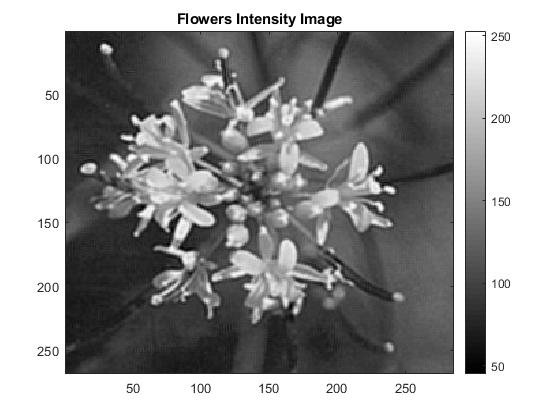
\includegraphics[width=55mm]{flowersIntensity.jpg}
}
\subfloat[]{
  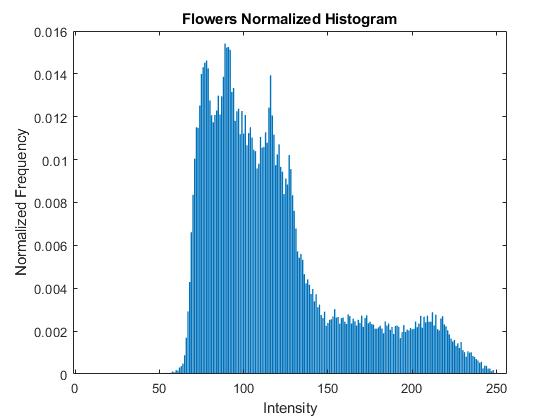
\includegraphics[width=55mm]{flowersNormHist.jpg}
}
\hspace{0mm}
\subfloat[]{
  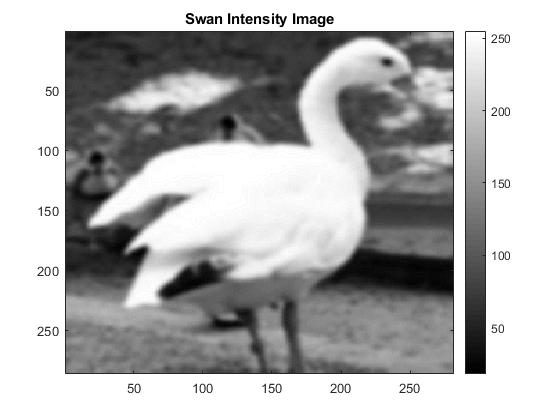
\includegraphics[width=55mm]{swanIntensity.jpg}
}
\subfloat[]{
  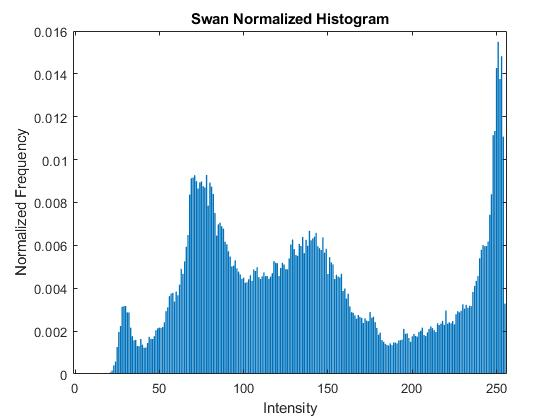
\includegraphics[width=55mm]{swanNormHist.jpg}
}
\hspace{0mm}
\subfloat[]{
  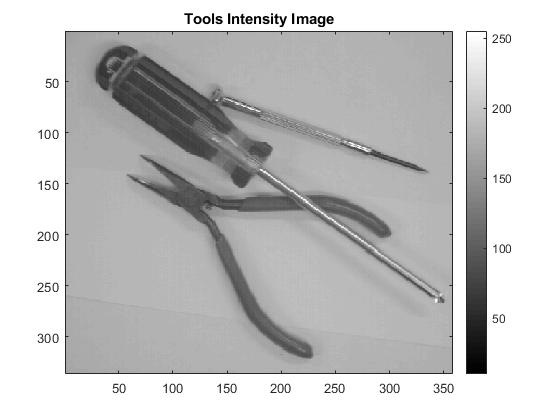
\includegraphics[width=55mm]{toolsIntensity.jpg}
}
\subfloat[]{
  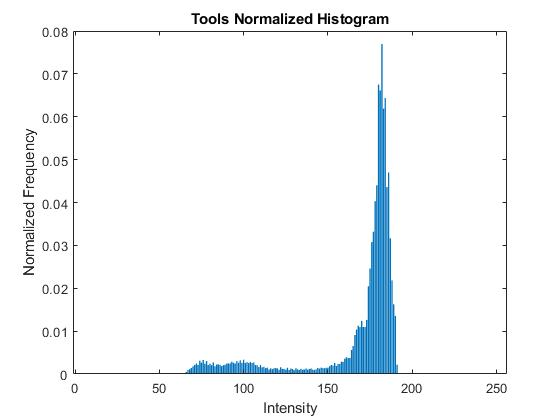
\includegraphics[width=55mm]{toolsNormHist.jpg}
}
\caption{Left Column: Original 8-bit Intensity Images Right Column: Normalized Histogram of Image Intensities}
\end{figure}

From the image histograms, the following inferences can be made about each image: 
\begin{itemize}
\item Flowers: Demonstrates low contrast, favors darker intensities
\item Swan: Shows more high-contrast characteristics than the other images
\item Tools: Exhibits low-contrast tendencies, favors lighter values
\end{itemize}

\newpage
\subsection*{myhisteq}

\begin{figure}[h!]
\captionsetup[subfloat]{labelformat=empty}
\centering
\subfloat[]{
  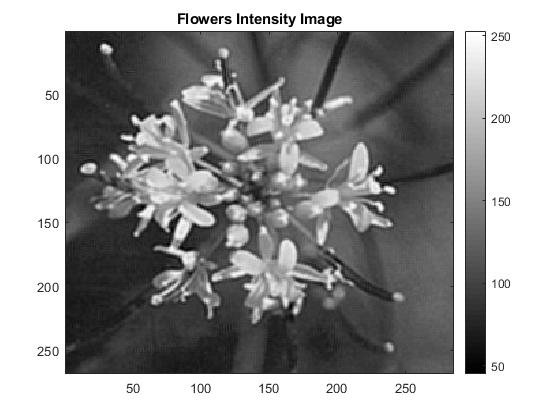
\includegraphics[width=35mm]{flowersIntensity.jpg}
}
\subfloat[]{
  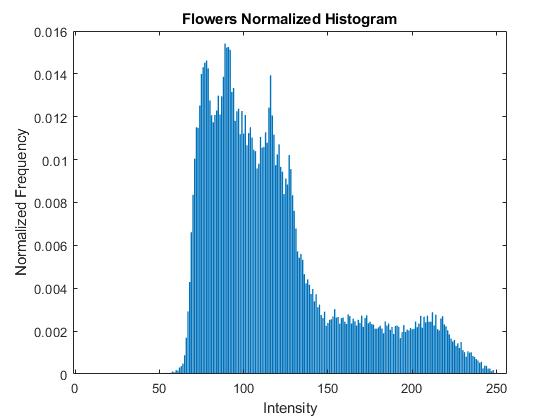
\includegraphics[width=35mm]{flowersNormHist.jpg}
}
\subfloat[]{
  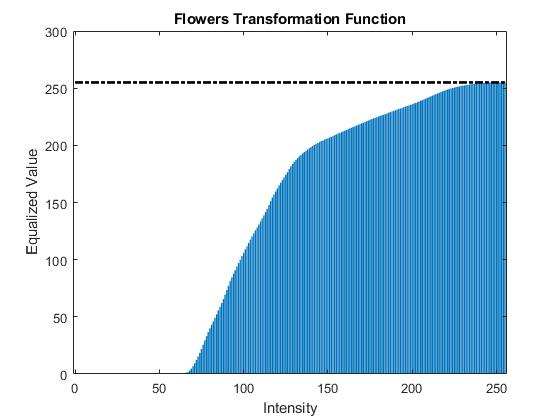
\includegraphics[width=35mm]{flowersEqTrans.jpg}
}
\subfloat[]{
  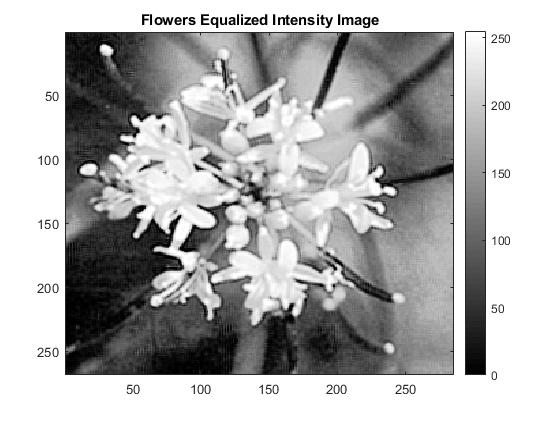
\includegraphics[width=35mm]{flowersIntensityEq.jpg}
}
\subfloat[]{
  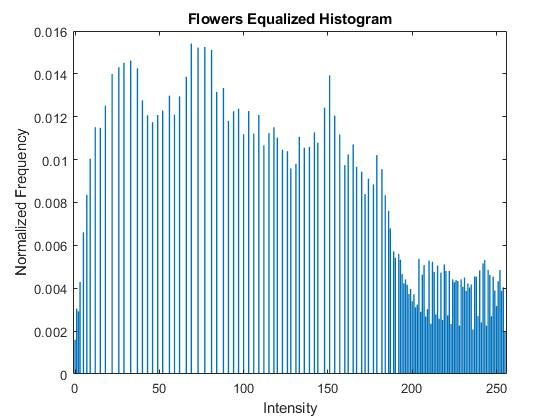
\includegraphics[width=35mm]{flowersNormHistEq.jpg}
}
\hspace{0mm}
\subfloat[]{
  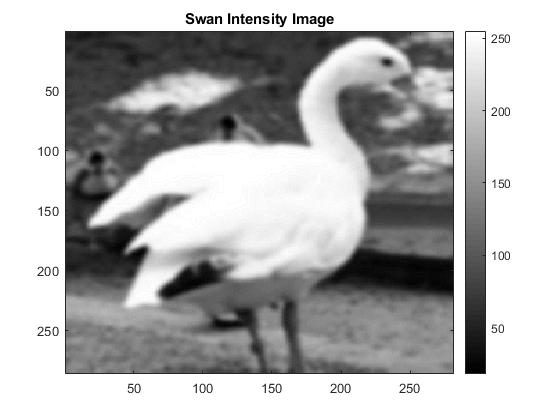
\includegraphics[width=35mm]{swanIntensity.jpg}
}
\subfloat[]{
  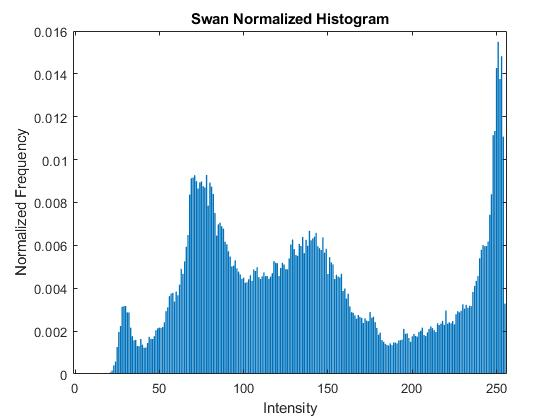
\includegraphics[width=35mm]{swanNormHist.jpg}
}
\subfloat[]{
  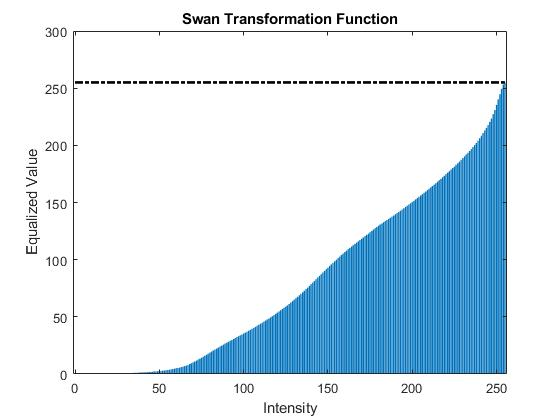
\includegraphics[width=35mm]{swanEqTrans.jpg}
}
\subfloat[]{
  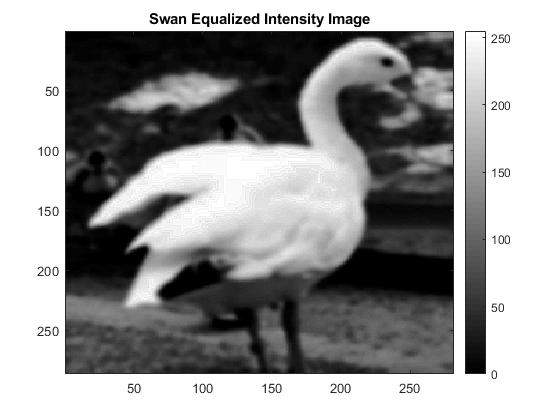
\includegraphics[width=35mm]{swanIntensityEq.jpg}
}
\subfloat[]{
  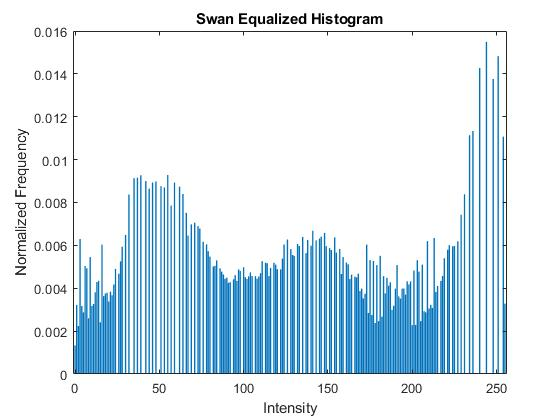
\includegraphics[width=35mm]{swanNormHistEq.jpg}
}
\hspace{0mm}
\subfloat[]{
  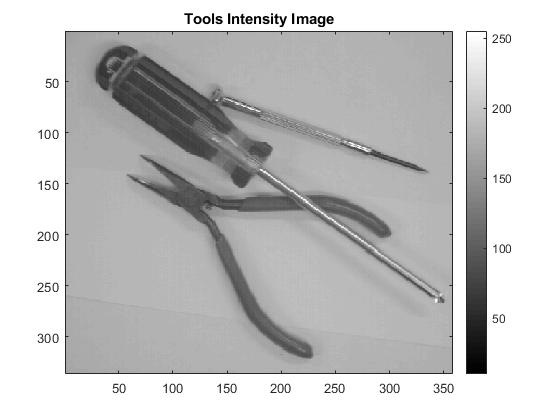
\includegraphics[width=35mm]{toolsIntensity.jpg}
}
\subfloat[]{
  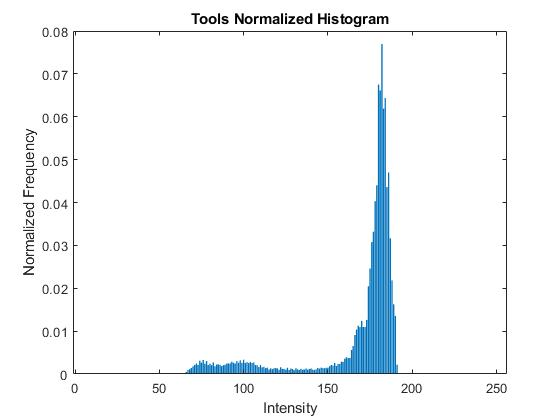
\includegraphics[width=35mm]{toolsNormHist.jpg}
}
\subfloat[]{
  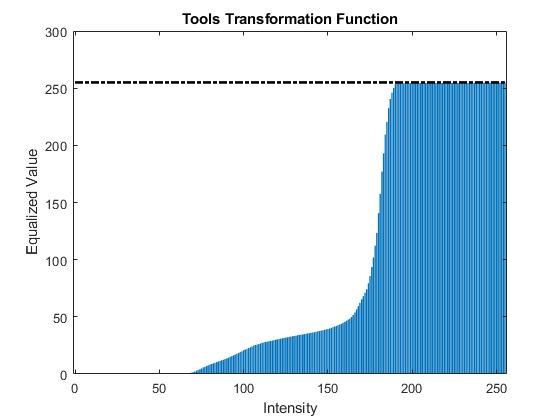
\includegraphics[width=35mm]{toolsEqTrans.jpg}
}
\subfloat[]{
  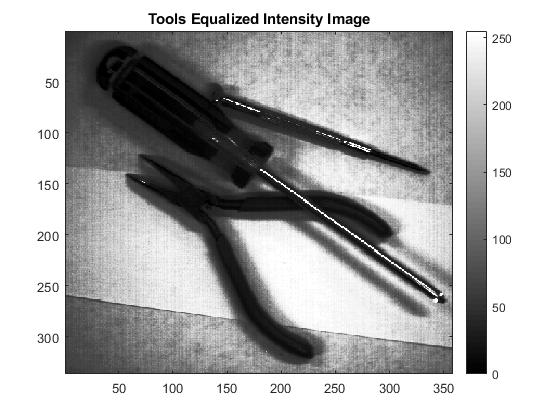
\includegraphics[width=35mm]{toolsIntensityEq.jpg}
}
\subfloat[]{
  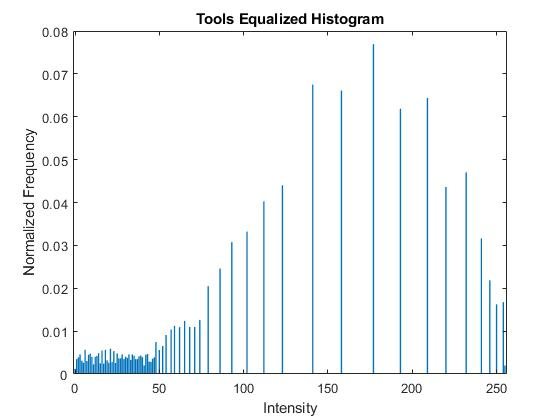
\includegraphics[width=35mm]{toolsNormHistEq.jpg}
}
\caption{Left to right columns: Original 8-bit Intensity Images,  Normalized Histogram of Image Intensities, Equalization Transformation Function, Equalized Intensity Image, Equalized Normalized Intensity Histogram}
\end{figure}

\noindent
The above images demonstrate the outputs of the \emph{myhisteq} function required for this assignment.  The differences between the original intensity images and the equalized images transformed by the shown equalization functions can be observed visually, as well as quantitatively through the normalized image intensity histograms.

\newpage
\subsection*{myquantize}
\begin{figure}[h!]
\captionsetup[subfloat]{labelformat=empty}
\centering
\subfloat[]{
  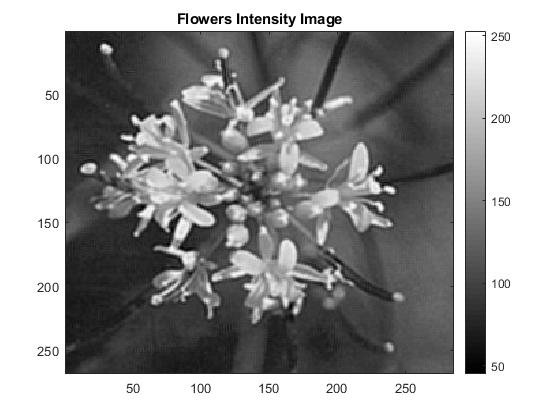
\includegraphics[width=40mm]{flowersIntensity.jpg}
}
\subfloat[]{
  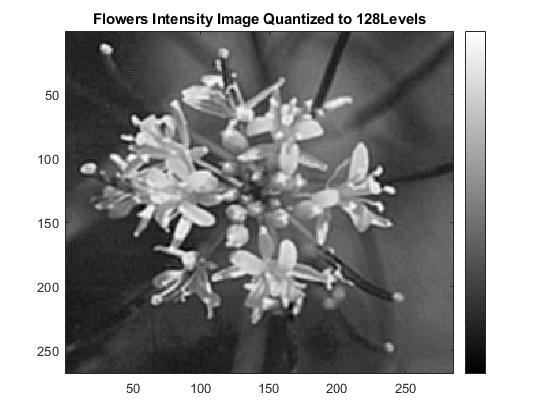
\includegraphics[width=40mm]{flowersQuant128.jpg}
}
\subfloat[]{
  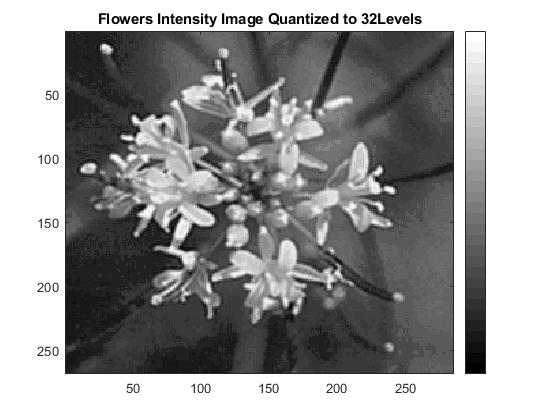
\includegraphics[width=40mm]{flowersQuant32.jpg}
}
\subfloat[]{
  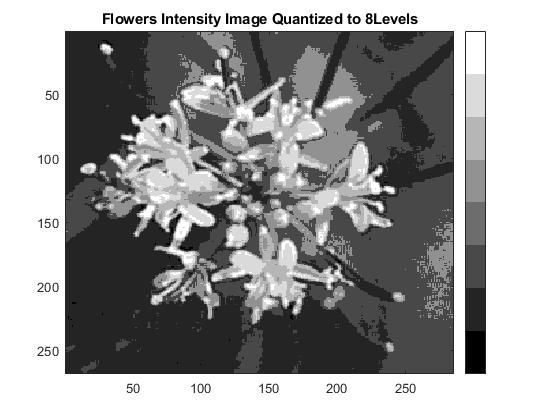
\includegraphics[width=40mm]{flowersQuant8.jpg}
}
\hspace{0mm}
\subfloat[]{
  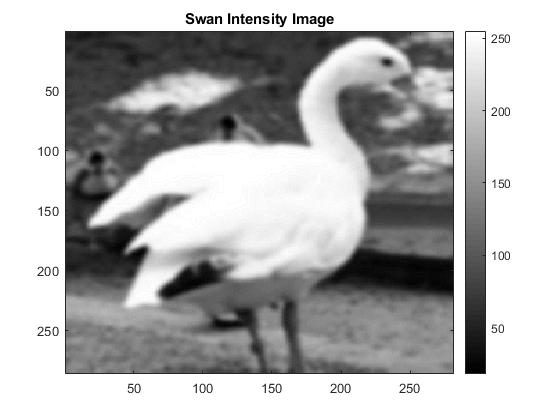
\includegraphics[width=40mm]{swanIntensity.jpg}
}
\subfloat[]{
  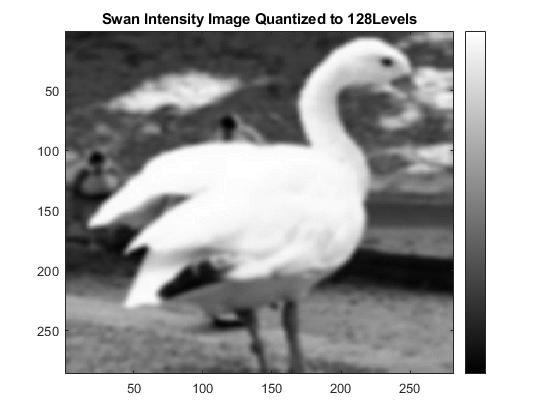
\includegraphics[width=40mm]{swanQuant128.jpg}
}
\subfloat[]{
  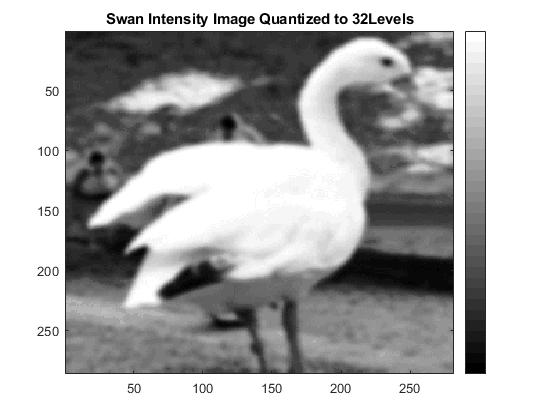
\includegraphics[width=40mm]{swanQuant32.jpg}
}
\subfloat[]{
  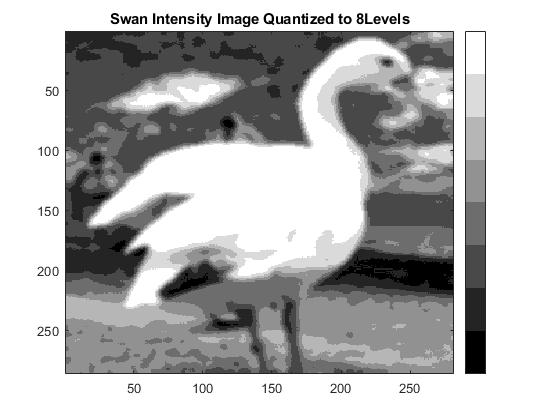
\includegraphics[width=40mm]{swanQuant8.jpg}
}
\hspace{0mm}
\subfloat[]{
  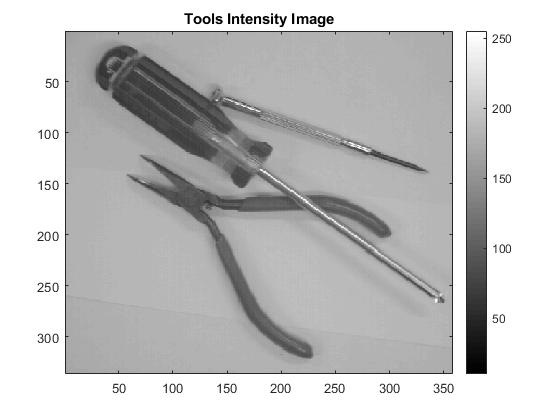
\includegraphics[width=40mm]{toolsIntensity.jpg}
}
\subfloat[]{
  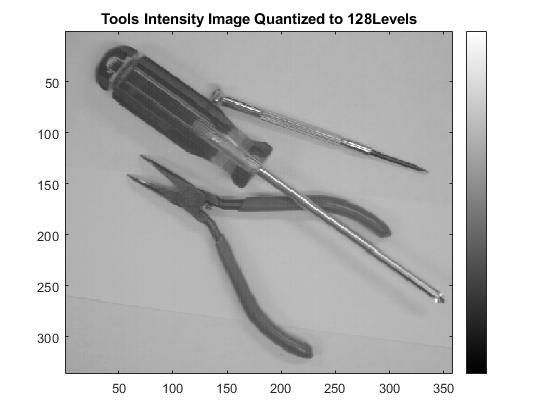
\includegraphics[width=40mm]{toolsQuant128.jpg}
}
\subfloat[]{
  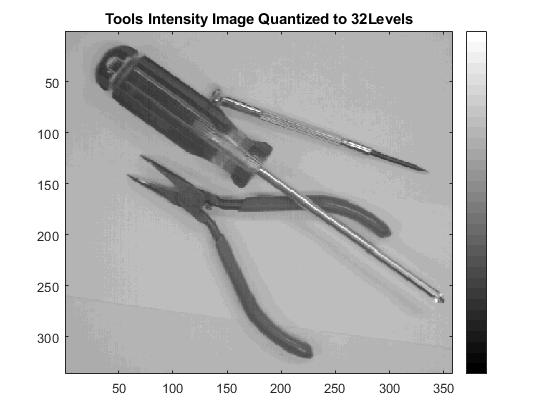
\includegraphics[width=40mm]{toolsQuant32.jpg}
}
\subfloat[]{
  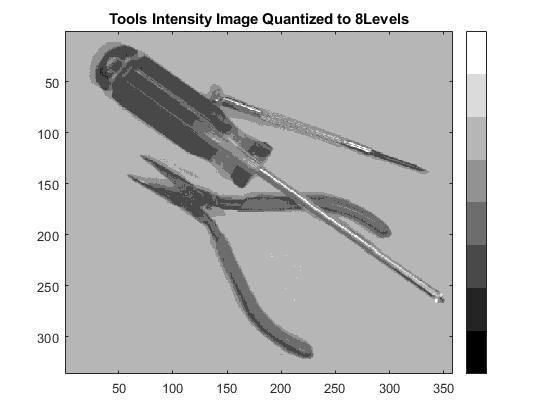
\includegraphics[width=40mm]{toolsQuant8.jpg}
}
\caption{From left to right: Original 8-bit Intensity image, Image quantized to 128 levels, Image quantized to 32 levels, Image quantized to 8 levels}
\end{figure}




\begin{algorithm}[H]
\caption{Quantization}\label{alg:quant}
\begin{algorithmic}[1]
\Procedure{Quantization}{}
\State $\textit{quantNum} \gets \text{number of intensity levels}$
\State $f \gets \textit{pixel intensity}$
\State $i \gets \textit{pixel index}$
\State $\textit{Q} \gets \textit{length of quantization intervals} = \frac{255}{quantNum}$
\For{i in numPixels}
\State $\textit{Index of quantized value}, Q_i(f_i) \gets \textit{floor}(\frac{f_i}{Q})$
\State $\textit{Quantized value}, Q_i(f_i) \gets Q_i(f_i)Q+\frac{Q}{2}$
\EndFor
\EndProcedure
\Return{Quantized Image}
\end{algorithmic}
\end{algorithm}
\vspace{5mm}
\noindent
The quantization function implemented for this assignment works as described in algorithm \ref{alg:quant}. \\
\noindent
In words, the space of possible intensities is divided into \textit{quantNum} regions.  Each pixel's intensity is classified into one of the regions.  Then each pixel's quantized value is set as the middle intensity value in its corresponding region.\\
 %===================================================================================================================
 
 \noindent 
 Accompanying code is provided in $mccurleyHW02.mat$


\end{document}
